%%
%% Copyright 2007-2025 Elsevier Ltd
%%
%% This file is part of the 'Elsarticle Bundle'.
%% Elsevier article template header
%%
%% It may be distributed under the conditions of the LaTeX Project Public
%% License, either version 1.3 of this license or (at your option) any
%% later version.  The latest version of this license is in
%%    http://www.latex-project.org/lppl.txt
%% and version 1.3 or later is part of all distributions of LaTeX
%% version 1999/12/01 or later.
%%
%% The list of all files belonging to the 'Elsarticle Bundle' is
%% given in the file `manifest.txt'.
%%
%% InventOR manuscript prepared with Elsevier's `elsarticle' class
%% using numbered bibliographic references.
%%
\documentclass[preprint,11pt]{elsarticle}

%% Use the option review to obtain double line spacing
%% \documentclass[authoryear,preprint,review,12pt]{elsarticle}

%% Use the options 1p,twocolumn; 3p; 3p,twocolumn; 5p; or 5p,twocolumn
%% for a journal layout:
%% \documentclass[final,1p,times]{elsarticle}
%% \documentclass[final,1p,times,twocolumn]{elsarticle}
%% \documentclass[final,3p,times]{elsarticle}
%% \documentclass[final,3p,times,twocolumn]{elsarticle}
%% \documentclass[final,5p,times]{elsarticle}
%% \documentclass[final,5p,times,twocolumn]{elsarticle}

%% For including figures, graphicx.sty has been loaded in
%% elsarticle.cls. If you prefer to use the old commands
%% please give \usepackage{epsfig}

%% The amssymb package provides various useful mathematical symbols
\usepackage{amssymb}
%% The amsmath package provides various useful equation environments.
\usepackage{amsmath}
\usepackage{enumitem}
\usepackage{array}
\usepackage{tabularx}
\usepackage[section]{placeins}
\usepackage{amsthm}
\usepackage{setspace}
\setstretch{1.5}
\newcolumntype{L}{>{\raggedright\arraybackslash}X}
\newcolumntype{P}[1]{>{\raggedright\arraybackslash}p{#1}}
\theoremstyle{plain}
\newtheorem{proposition}{Proposition}[section]
\newtheorem{corollary}{Corollary}[proposition]
\setlength{\emergencystretch}{3em}
\setlength{\textfloatsep}{8pt plus 2pt minus 2pt}
\setlength{\intextsep}{8pt plus 2pt minus 2pt}
\setlength{\abovecaptionskip}{4pt}
\setlength{\belowcaptionskip}{2pt}
\setcounter{topnumber}{3}
\setcounter{bottomnumber}{2}
\setcounter{totalnumber}{5}
\renewcommand{\topfraction}{0.9}
\renewcommand{\bottomfraction}{0.8}
\renewcommand{\textfraction}{0.07}
\renewcommand{\floatpagefraction}{0.8}
\hfuzz=20pt
\hbadness=10000
%% The amsthm package provides extended theorem environments
%% \usepackage{amsthm}

\usepackage{lineno}

\journal{Omega}

\begin{document}

\begin{frontmatter}

%% Title, authors and addresses

%% use the tnoteref command within \title for footnotes;
%% use the tnotetext command for theassociated footnote;
%% use the fnref command within \author or \affiliation for footnotes;
%% use the fntext command for theassociated footnote;
%% use the corref command within \author for corresponding author footnotes;
%% use the cortext command for theassociated footnote;
%% use the ead command for the email address,
%% and the form \ead[url] for the home page:
%% \title{Title\tnoteref{label1}}
%% \tnotetext[label1]{}
%% \author{Name\corref{cor1}\fnref{label2}}
%% \ead{email address}
%% \ead[url]{home page}
%% \fntext[label2]{}
%% \cortext[cor1]{}
%% \affiliation{organization={},
%%             addressline={},
%%             city={},
%%             postcode={},
%%             state={},
%%             country={}}
%% \fntext[label3]{}

\title{InventOR: A Prompt-Configured, No-Fine-Tuning LLM Workflow for Material-Level Inventory Control}

%% use optional labels to link authors explicitly to addresses:
%% \author[label1,label2]{}
%% \affiliation[label1]{organization={},
%%             addressline={},
%%             city={},
%%             postcode={},
%%             state={},
%%             country={}}
%%
%% \affiliation[label2]{organization={},
%%             addressline={},
%%             city={},
%%             postcode={},
%%             state={},
%%             country={}}

\author[inst1]{Aris Dressino\corref{cor1}} %% Author name
\cortext[cor1]{Corresponding author. Telephone: +49 89 289 25000.}
\ead{aris.dressino@tum.de}

%% Author affiliation
%% Department of Advanced Analytics in Manufacturing Management
\affiliation[inst1]{organization={TUM School of Management, Technical University of Munich},%Department and Organization
            addressline={Arcisstraße 21},
            city={Munich},
            postcode={80333},
            country={Germany}}

%% Abstract
\begin{abstract}
This paper presents \emph{InventOR}, a prompt-configured large-language-model (LLM) workflow for material-level inventory decision support under demand and lead-time uncertainty. A material-scoped historical CSV and inline parameter block are supplied through an enterprise LLM application; no project-specific model weights were trained or fine-tuned on enterprise data. The LLM returns a policy artifact that deterministic parsing and simulation evaluate against an SAP-derived comparator and an SAP-safety-lead-time-informed operations-research $(r,Q)$ comparator. The LLM is therefore a candidate-policy generator, not an autonomous ERP controller. The executed artifact set covers all 365 eligible plant-material pairs in a three-plant industrial dataset after retry handling and capacity validation. A common-feasible cohort of 346 pairs applies identical MOQ and per-material storage rules to all arms. Working-day post-cutoff simulation reports 77.52\% demand-weighted aggregate fill, 97.94\% mean material fill, and 2{,}848.96 mean simulated material-horizon holding/order cost for the LLM-emitted arm. Positive lost-sales penalty sensitivities remove its apparent cost advantage. These values remain descriptive simulated comparison rather than controlled production-trial evidence. Stored metadata do not establish the exact deployed prompt or model/runtime identity; the contribution is a transparent prototype workflow and disclosure of controls required for prospective evaluation.
\end{abstract}

%% Keywords
\begin{keyword}
Generative Artificial Intelligence \sep Large Language Models \sep Operations Research \sep Supply Chain Management \sep Decision Support Systems \sep Explainable AI \sep Inventory Control
\end{keyword}

\end{frontmatter}

\linenumbers

%% main text
%%

\section{Introduction}
\label{sec:intro}

Supply chain planning operates under volatile demand, uncertain replenishment, and disruption exposure \cite{sengupta2025uncertainty}. Many material-control decisions nevertheless still depend on simple parameters: reorder points, safety stock, order quantities, review periods, and sometimes safety lead time; these settings strongly affect service and inventory exposure \cite{grasso1984simulation, vanKampen2010safety}. Classical operations research offers rigorous tools for stochastic and robust inventory decisions \cite{bertsimas2006robust, thorsen2017robust, zhang2025robust}, but operational planners often need a narrower capability: converting imperfect historical records into transparent, defensible, and auditable material-level policy values \cite{mersereau2013information}.

Large language models (LLMs) can help connect business intent, operational evidence, and analytical workflows \cite{boone2025generative, wasserkrug2025enhancing}. In inventory control, however, recommendations require explainability, reproducibility, accountability, and meaningful human control before planners can act on them \cite{amershi2019guidelines, raji2020accountability}. This creates a practical design requirement for hybrid AI-supported OR systems: LLM artifacts must be inspectable, while their numeric recommendations require explicit simulation and human release controls \cite{wasserkrug2025enhancing, raji2020accountability}.

This paper addresses that requirement through \emph{InventOR}, an operations-research-first workflow for material-level inventory decision support. An enterprise LLM application produces policy artifacts from material-scoped inputs; deterministic software parses and simulates their numeric values. The study evaluates independent plant-material pairs, not shared-capacity inventory control, and does not estimate implementation cost or planner adoption.

The contribution of this paper is an evaluation protocol rather than a new inventory model or solution algorithm. The comparator policies are standard textbook constructions; what the paper adds is a reusable, auditable procedure for deciding whether LLM-emitted policy values are admissible and how they perform against ERP-derived baselines on a common simulation horizon. Three components make up that protocol.

\begin{enumerate}[label=\textbf{C\arabic*}, leftmargin=2.2em, itemsep=3pt]
\item \textbf{Admissibility protocol for LLM-emitted policy artifacts.} Material-specific inputs pass through a configured enterprise LLM application without project-specific training or fine-tuning. Deterministic scoreability and capacity checks decide admission; the architecture reserves a planner release step, which this study documents as a design requirement rather than an evaluated intervention \cite{sahoo2024systematic}.
\item \textbf{Executable boundary specification.} The paper documents the material-input contract, alias-aware conversion, capacity validation, and simulation boundary, so that a competing generator can be substituted and scored under identical rules.
\item \textbf{Complete-cohort reporting discipline.} All 365 eligible pairs from 233{,}078 parsed records yielded scoreable, capacity-feasible artifacts after retry handling; 346 pairs meet the common feasibility rules used for the three-arm descriptive comparison. No pair is silently dropped, and every exclusion rule is prespecified and reported.
\end{enumerate}

The remainder of the paper reviews related work, presents the executed workflow and policy logic, reports exploratory post-cutoff simulation results, and discusses the controls needed before a valid deployment evaluation.

\section{Literature Review}
\label{sec:literature}

Operations research has long addressed supply-chain uncertainty through stochastic programming, robust optimization, and scenario-based planning \cite{bertsimas2006robust, thorsen2017robust, zhang2025robust}. These methods formalize variability and recourse, but operational inventory teams often face a more direct implementation problem: maintaining reorder points, safety stock, safety lead time, and order quantities from incomplete historical evidence in ERP-driven planning environments \cite{silver2017inventory, zipkin2000foundations, grasso1984simulation, vanKampen2010safety}. Static rules can be too coarse, while sophisticated models can be difficult to explain and maintain. This motivates decision support that keeps OR discipline while making material-level parameter setting more transparent and auditable \cite{mersereau2013information, kang2005information}.

Recent LLM research proposes natural-language interfaces, tool-using agents, and pipelines that translate natural-language requests into optimization model structures or executable code \cite{wasserkrug2025enhancing, huang2025orlm, cohen2025supply, ahmaditeshnizi2024optimus}. Published conceptual systems and recent preprints illustrate a rapidly evolving frontier, including multi-agent LLM systems that make autonomous per-period inventory decisions \cite{pinto2024conversationally, zhang2025or, quan2025invagent}. They do not by themselves specify how inventory histories should be reduced into demand regimes, lead-time diagnostics, service buffers, and feasible policy parameters. Prior work therefore supports the hybrid position adopted here: LLM artifacts can structure workflows and explanations, while deterministic parsing and simulation make their consequences inspectable and planners retain decision authority \cite{wasserkrug2025enhancing, amershi2019guidelines}.

InventOR follows this hybrid view. It supplies one filtered historical CSV for the focal material plus an inline parameter block through an enterprise LLM application. The intended prompt specification prohibits stochastic simulation, machine-learning libraries, and unrestricted data fabrication, but the stored run metadata do not independently identify the deployed prompt or runtime. Because LLM outputs can contain fabricated or unfaithful content \cite{ji2023survey}, the executed downstream parser uses alias-aware lookups and nested-field resolution before requiring numeric positive reorder point and order quantity, numeric non-negative safety stock, and a resolvable simulator family. No project-specific model fitting or fine-tuning is performed. The design treats the LLM as an artifact-generation component inside a bounded decision process. Table~\ref{tab:literature-positioning} positions the framework relative to recent AI-supported OR and inventory-control work.

\begin{table}[htbp]
\centering
\caption{Literature positioning: InventOR relative to recent AI-supported OR contributions for inventory and supply chain decision support.}
\label{tab:literature-positioning}
\scriptsize
\setlength{\tabcolsep}{2pt}
\renewcommand{\arraystretch}{1.10}
\begin{tabularx}{\textwidth}{p{2.1cm} p{1.55cm} p{1.75cm} p{1.65cm} p{1.85cm} L}
\hline
\textbf{Study} & \textbf{LLM role} & \textbf{Policy class} & \textbf{Demand model} & \textbf{Analytical result} & \textbf{Evaluation} \\
\hline
Huang et al.~\cite{huang2025orlm} & NL$\to$code & General OR & Not specified & None & Benchmark \\
Ahmaditeshnizi et al.~\cite{ahmaditeshnizi2024optimus} & NL$\to$model & General OR & Not specified & Solver-linked & Benchmark \\
Zhang et al.~\cite{zhang2025or} & Reasoning agent & General OR & Not specified & Model and solve & Case studies \\
Quan and Liu~\cite{quan2025invagent} & Multi-agent control & Inventory & Sequential demand & Per-period decisions & Simulation \\
Prak et al.~\cite{prak2021robust} & None & Inventory control & Compound Poisson / intermittent & Robust estimation & Empirical study \\
Babai et al.~\cite{babai2026fifty} & None & Forecasting-linked inventory & Regime-specific & Review synthesis & Review \\
Wasserkrug et al.~\cite{wasserkrug2025enhancing} & Interface & General & Not specified & None & Conceptual \\
Cohen et al.~\cite{cohen2025supply} & Vision & General SCM & Not specified & None & Vision statement \\
\textbf{InventOR} & \textbf{Prototype} & \textbf{$(r,Q)$ executed; $(s,S)$ implemented, unexercised} & \textbf{Artifact-defined values} & \textbf{Descriptive} & \textbf{Post-cutoff simulation} \\
\hline
\end{tabularx}
\end{table}
\FloatBarrier

The table highlights the paper's narrower contribution: material-level parameter artifacts evaluated by a deterministic policy-family simulator. Unlike InvAgent's sequential multi-agent decisions, InventOR emits one stationary policy per material from a bounded historical package; unlike OptiMUS and OR-LLM-Agent, it does not formulate or solve general optimization models.

\section{Methodology}
\label{sec:method}

The unit of analysis is a plant-material pair. The framework records a chain of custody from historical records to planner-facing policy values by separating deterministic input preparation, configured LLM inference, schema parsing, deterministic simulation, and human review \cite{mersereau2013information, watts2009data}. Each LLM session receives one filtered, material-scoped historical CSV as a session resource and a small inline parameter block containing current cost, MOQ, service, SAP reference, and material-level storage-capacity fields. No project-specific model weights are trained, fine-tuned, or updated. Because the stored metadata omit prompt hash, application version, and model/runtime identifier, this study does not claim that the exact deployed instruction configuration is independently reproducible. Supplementary File S1 reproduces the intended application-side system and tool prompt texts verbatim, together with their disclosed discrepancies against the executable simulator.

\subsection{Problem Definition: Single-Item Continuous-Review Control with Stress-Adjusted Service Buffering}
\label{subsec:problem-framing}

The executed task is a single-item, single-echelon continuous-review simulation with lost sales \cite{silver2017inventory, zipkin2000foundations, bijvank2011lost}. Each plant-material pair is treated independently; multi-item coupling, shared capacity, substitution, and production scheduling are outside the pilot. For the SAP-SLT-informed OR comparator, pre-cutoff working-day demand yields mean demand $\bar d_i$, annualized demand $\bar D_i^{\mathrm{ann}}=250\bar d_i$, lead-time-demand dispersion, and stationary $(R_i,Q_i)$ parameters. This comparator is not independent of ERP inputs because source SAP safety lead time enters effective lead time. For the SAP-derived arm, source safety stock is retained while $R_i$ and $Q_i$ are recomputed by the same executable routines. For the LLM arm, scoreable policy parameters originate directly in the artifact and pass alias-aware compatibility parsing plus strict executable-contract validation; the reference equations below do not reconstruct them. The simulator executes validated $(r,Q)$ artifacts as fixed-quantity policies and validated $(s,S)$ artifacts as order-up-to policies. In this study all 365 scoreable artifacts resolved to the $(r,Q)$ family after validation, so the order-up-to path is an available but unexercised capability rather than an evaluated result.

\paragraph{Reference policy calculation}
The following equations describe the executed SAP-SLT-informed OR comparator; they do not reconstruct direct LLM-emitted policies. The order quantity $Q_i>0$ is rounded upward to an integer, floored at source MOQ, and then projected to its material-level storage limit when possible. The reorder point $R_i\ge0$ triggers replenishment. The EOQ anchor minimizes the standard annual cost approximation
\[
\min_{Q_i}\;TC_i\!\left(Q_i;\,SS_i\right)=h_i\!\left(\frac{Q_i}{2}+SS_i\right)+K_i\frac{\bar D_i^{\mathrm{ann}}}{Q_i},
\]
where $SS_i$ is arm-specific safety stock, $h_i=\texttt{holding\_cost\_rate}_i\cdot\texttt{unit\_cost}_i$, and $K_i=\texttt{ordering\_cost}_i$. The implementation first uses $Q_i=\max\{\mathrm{MOQ}_i,\lceil\sqrt{2K_i(250\bar d_i)/h_i}\rceil\}$ when demand and ordering cost are positive, and MOQ otherwise. For every arm, a supplied capacity requires $\mathrm{MOQ}_i\leq Q_i$ and $SS_i+Q_i\leq\texttt{max\_storage\_units}_i$; comparator quantities above the residual limit are reduced, while pairs with $SS_i+\mathrm{MOQ}_i$ above the limit are excluded from the common cohort. The SAP-SLT-informed OR safety stock is $SS_i=\lceil z_{\alpha_i}\sigma_{LTD,i}\rceil$, with $R_i=\lceil\bar d_iL_i^{\mathrm{eff}}+SS_i\rceil$. The SAP-derived arm substitutes source SAP safety stock into the same reorder-point expression. No lot-size multiple or stress coefficient is executed. The primary holding/order cost has a zero shortage penalty; positive lost-sales penalties are sensitivity analyses.

\paragraph{Core constraints}
Inventory evolves under a lost-sales continuous-review rule on the working-day decision set $\mathcal{W}$. All arms share the first observed post-cutoff on-hand inventory; the SAP-SLT-informed OR $R_i+Q_i$ is used only when that observation is unavailable. The initial on-order pipeline is empty. Duplicate same-material, same-date rows are aggregated by summing demand, receipts, corrections, and scrap and averaging positive lead times, but the simulator consumes only demand and excludes observed receipts, corrections, and scrap. The simulator rounds mean source lead time and schedules every modeled order by that number of subsequent working observations:
\[
I_{i,t}=\max\!\left(0,\;I_{i,t-1}+a_{i,t}-d_{i,t}\right),\quad t\in\mathcal{W},
\]
where $a_{i,t}$ is the quantity whose working-day due observation is no later than $t$. Scheduled arrivals are added first, realized demand is served subject to lost sales, and the post-demand inventory position is computed as on-hand plus outstanding orders. For a validated $(r,Q)$ artifact, a fixed quantity is ordered when
\[
\delta_{i,t}=\mathbf{1}\{\mathrm{IP}_{i,t}^{+}\le R_i\},
\qquad
\mathrm{IP}_{i,t}^{+}=I_{i,t}+\sum_{s:\,\mathrm{due}(s)>t}o_{i,s},
\]
with $o_{i,t}=Q_i\delta_{i,t}$. For a validated $(s,S)$ artifact, the same threshold test uses $s_i$, and an order of $S_i-\mathrm{IP}_{i,t}^{+}$ is placed when positive; no artifact in this study triggered that branch. Orders due after the observed horizon remain in transit rather than being forced onto the final observation. Parameters remain stationary. Shared observed initialization and the empty initial pipeline are part of the executed comparison design.

The reorder point targets a nominal cycle service level $\alpha_i\in[0.5,0.999]$ after numeric clamping. Under the normal approximation,
\[
\mathbb{P}\!\left(D_{i,L_i^{\mathrm{eff}}}\le R_i\right)\ge\alpha_i
\;\Longleftrightarrow\;
R_i\ge\bar d_i L_i^{\mathrm{eff}}+z_{\alpha_i}\,\sigma_{LTD,i}.
\]
The reported backtest metric is the ex-post fill rate, which is distinct from the nominal cycle-service target because it also depends on $Q_i$ and realized demand \cite{axsater2015inventory}.

Lead-time-demand variance is propagated under the demand and lead-time independence approximation,
\[
\sigma_{LTD,i}^2=L_i^{\mathrm{eff}}\sigma_{D,i}^2+\bar d_i^2\sigma_{L,i}^2.
\]
The executed SAP-SLT-informed OR buffer is
\[
SS_i^{\mathrm{OR}}=z_{\alpha_i}\sigma_{LTD,i},
\]
with values rounded upward:
\[
SS_i^{\mathrm{OR}}=\left\lceil z_{\alpha_i}\sigma_{LTD,i}\right\rceil,
\qquad
R_i=\left\lceil\bar d_iL_i^{\mathrm{eff}}+SS_i^{\mathrm{OR}}\right\rceil.
\]
The executable statistics add non-negative source SAP safety-lead-time days to mean lead time when constructing comparator lead-time-demand dispersion (Section~\ref{subsec:slt} discusses this confound). LLM-emitted values remain artifact values accepted by alias-aware parsing and strict executable-contract validation.

\paragraph{Parser and review boundary}
Artifact policy labels determine simulator routing after validation. The parser resolves compatibility aliases, then requires a valid $(r,Q)$ tuple or explicit $s$ and $S$ values for an $(s,S)$ label; it rejects malformed, infeasible, or internally inconsistent artifacts. It does not execute label-specific optimization or deterministic escalation. Because no artifact supplied explicit and internally consistent $s$ and $S$ values, every scored policy in this study was executed as $(r,Q)$; the reported evidence therefore concerns fixed-quantity control only. Planner review remains required before any operational use.

Methodologically, the contribution is therefore not to replace OR with an LLM. Rather, it is an integration of deterministic input preparation, configured LLM artifact generation, schema parsing, and explicit policy simulation in a single prototype workflow \cite{amershi2019guidelines, raji2020accountability}.

\subsection{Historical Input Schema and Canonical Analysis Table}
\label{subsec:data-schema}

The source table is grouped by plant and material, but the uploaded material CSV contains only the subset listed in Table~\ref{tab:lt-schema}. Plant and material identifiers are carried by the run key and inline block rather than repeated in the uploaded rows. The inline block also passes current cost, MOQ, service, SAP reference, working-day demand, lead-time, and material-level storage-capacity variables. Deterministic preprocessing supplies input normalization, eligibility filters, and simulator statistics. Stock-flow fields omitted from the uploaded subset are not analyzed by the executed LLM path.

\begin{table}[htbp]
\centering
\caption{Fields included in the material-scoped CSV uploaded by the executed runner.}
\label{tab:lt-schema}
\scriptsize
\setlength{\tabcolsep}{2pt}
\renewcommand{\arraystretch}{1.03}
\begin{tabularx}{\textwidth}{@{}P{3.35cm} P{1.15cm} L@{}}
\hline
\textbf{Column} & \textbf{Type} & \textbf{Description and method use} \\
\hline
\texttt{date} & date / datetime & Calendar observation date; time ordering, aggregation, and diagnostics \\
\texttt{actual\_demand} & numeric & Realized demand; mean, variability, intermittency, trend, and regime classification \\
\texttt{delivery\_time} & numeric & Recorded replenishment lead time; rounded and scheduled as subsequent working observations by the simulator \\
\texttt{minimum\_order\_quantity} & numeric & Minimum replenishment quantity; order-size feasibility constraint \\
\texttt{safety\_stock\_units} & numeric & Existing safety stock; benchmarking against computed recommendations \\
\texttt{safety\_time\_}\linebreak\texttt{workdays\_actual} & numeric & Source SAP safety-lead-time field; currently enters comparator effective lead time \\
\texttt{supplier\_plant\_}\linebreak\texttt{distance} & numeric & Supplier-to-plant distance; contextual lead-time-risk information \\
\texttt{reliability\_calc} & numeric & Source supplier or lane reliability context \\
\texttt{transportation\_network} & string & Source transportation-network context \\
\texttt{service\_level\_target} & numeric & Source service target used by comparator calculations \\
\texttt{unit\_cost} & numeric & Purchase or standard cost per unit in the source dataset's internal cost denomination; inventory-value proxy and input to holding-cost derivation and EOQ calculation \\
\texttt{holding\_cost\_rate} & numeric & Annual carrying-cost rate as a decimal (e.g., 0.20 for 20\% of unit value); used to derive the annual cost of carrying one unit in stock, balance replenishment frequency against stock exposure, and compute economic order quantity \\
\texttt{ordering\_cost} & numeric & Fixed replenishment cost in the source dataset's internal cost denomination; input to EOQ calculation and simulated material-horizon holding/order cost \\
\texttt{max\_storage\_units} & numeric & Material-level upper bound applied to all evaluated arms: $\mathrm{MOQ}\leq Q$ and $SS+Q\leq\texttt{max\_storage\_units}$ \\
\texttt{is\_working\_day} & binary & Working-day flag; working-day demand statistics and non-zero demand share \\
\hline
\end{tabularx}
\end{table}
\FloatBarrier

\subsection{Analytical Workflow}
\label{subsec:workflow}

The workflow transforms a historical material snapshot into a policy artifact through deterministic preparation, LLM inference, parsing, and simulation (Figure~\ref{fig:tool_process_map}).

\begin{figure}[htbp]
  \centering
  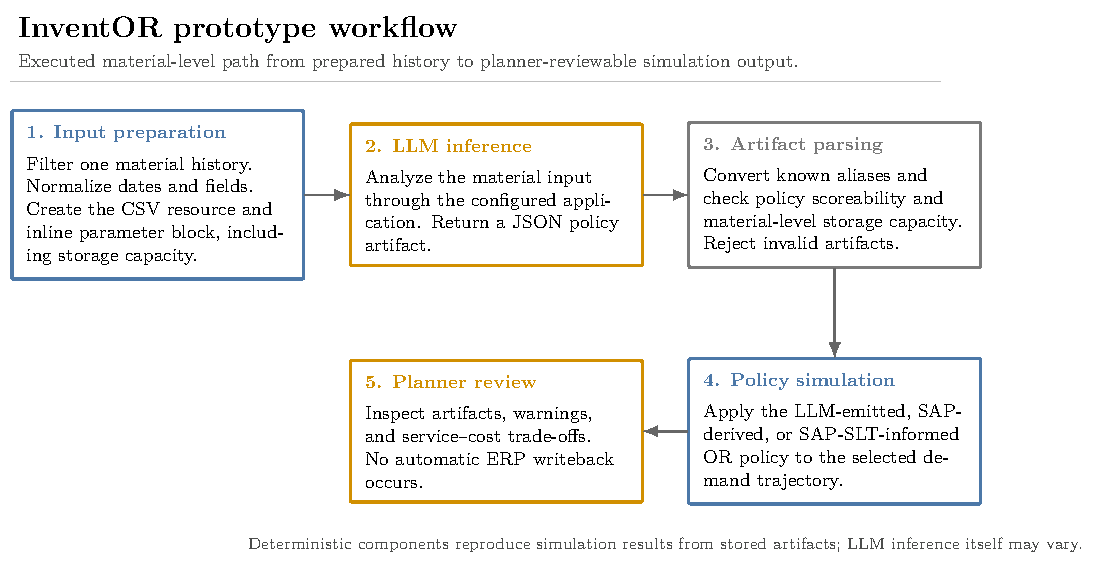
\includegraphics[width=0.92\linewidth]{Figure_1_Workflow.pdf}
\caption{Prototype workflow from material input preparation to policy artifact and simulation output.}
  \label{fig:tool_process_map}
\end{figure}
\FloatBarrier

The runner uploads a normalized material CSV and inline block; the configured application returns a JSON artifact. The parser converts accepted fields to an executable $(r,Q)$ or $(s,S)$ policy and rejects malformed or infeasible outputs. Missing or invalid artifacts are recorded and retried. The simulator evaluates accepted LLM values, SAP-derived values, and the SAP-SLT-informed OR policy on the common horizon. An aggregate-only manifest records active-input, evaluation-code, and stored-artifact hashes; it explicitly records unavailable historical deployed prompt, application, model/runtime, setting, and timestamp metadata. Current runner code records these fields for future runs when the corresponding environment variables are supplied. The author declares retrospectively that the evaluated artifacts were produced with an Anthropic Claude Sonnet 4.6 model behind the enterprise application, using a code-interpreter style Python execution tool; this declaration is recorded in the manifest as unverified because no deployed model identifier or generation settings were persisted at run time, and it must not be read as machine-verified provenance. Stored inputs, artifacts, and code reproduce a recorded simulation, but not a fresh LLM completion; planners retain implementation authority.

\subsection{Artifact Completeness and Future Readiness}
\label{subsec:validation}

The completeness audit asks whether each eligible pair has a scoreable artifact after retries; it does not estimate first-pass reliability, explanation completeness, or deployment readiness. The empirical section is a retrospective audit of an already-executed workflow rather than a controlled experiment: the generation cohort was produced before the evaluation protocol was finalized, the deployed configuration was not frozen or instrumented in advance, and no treatment was assigned. The post-cutoff simulation uses artifacts generated exclusively from pre-cutoff inputs and is descriptive rather than a controlled prospective trial \cite{tashman2000out, hewamalage2023forecast}. A future evaluation must freeze the deployed configuration, model/runtime identifiers, access controls, and approval workflow.

\subsection{Safety Lead Time Computation}
\label{subsec:slt}

Safety lead time (SLT) is an ancillary ERP-facing design field. The prototype specification proposes combining transport, supplier, and quality lead-time variability with a reliability-deficit premium \cite{silver2017inventory, vanKampen2010safety}, but the present release does not document estimators for those components. In the executed comparator code, non-negative source SAP safety-lead-time days are added to mean lead time before computing both SAP-derived and OR-computed dispersion and reorder points (this coupling is also flagged in Section~\ref{subsec:problem-framing}). The OR arm is therefore labelled SAP-SLT-informed, and no separate SLT effect is identified.

\subsection{Post-Cutoff Policy Simulation}
\label{subsec:backtest-design}

The confidential operational extract contains 233{,}078 parsed CSV records, 411 plant-material pairs, and three anonymized plants (Plant A, Plant B, and Plant C). The parameter cutoff is 2026-03-10 and the post-cutoff simulation horizon ends on 2026-08-27. Eligibility filters retain 365 plant-material pairs with sufficient pre-cutoff and post-cutoff evidence: 234 from Plant A, 65 from Plant B, and 66 from Plant C. Plant C has no positive source working-day flags, so its calendar flags are derived from same-date Plant A and Plant B votes; ties classify as working days. This deterministic repair permits a common decision calendar; because no alternative Plant C calendar exists, robustness is examined by reporting calendar-day arrivals and by re-running the full comparison on the native-calendar subset that excludes Plant C entirely. SAP-derived and SAP-SLT-informed OR parameters use pre-cutoff information. Stored LLM artifacts were generated from cutoff-bounded pre-cutoff inputs, so every arm is evaluated on the same post-cutoff horizon. Nineteen pairs cannot meet comparator safety stock plus MOQ within their supplied capacity; these are excluded before the common 346-pair comparison.

The simulated arms are: (i) SAP-derived, retaining source SAP safety stock while recomputing reorder point and EOQ order quantity from pre-cutoff statistics; (ii) SAP-SLT-informed OR, using the same statistics, source safety-lead-time input, and feasibility rules but without LLM inference; and (iii) LLM-emitted, a validated $(r,Q)$ or $(s,S)$ artifact. The simulator is continuous-review and lost-sales: all arms begin with the same first observed post-cutoff on-hand inventory, using the OR $ROP+Q$ only as a shared fallback. The initial on-order pipeline is empty. On each working row, modeled arrivals due after rounded mean working-day lead time are received, demand is served subject to lost sales, post-demand inventory position is checked, and a policy-specific order is placed if its threshold is met. Observed post-cutoff receipts, corrections, and scrap are excluded. This common startup design may create cutoff transients. Metrics are fill rate, aggregate demand-weighted fill rate, materials above 95\% fill, zero-stockout materials, stockout days, average on-hand inventory, and simulated material-horizon cost.

For policy $p$ and material $i$, the cost summaries use the simulated horizon of $T_i$ working days. Let $\overline{I}_{i,p}$ be average on-hand inventory, $h_i$ annual holding cost per unit, $K_i$ fixed ordering cost, and $n^{\mathrm{orders}}_{i,p}$ simulated orders. The implementation uses a constant 250 annual working days and computes
\[
TC_{i,p}=h_i\overline{I}_{i,p}\frac{T_i}{250}+K_i n^{\mathrm{orders}}_{i,p}.
\]
This is a simulated material-horizon holding/order cost in the source dataset's internal cost denomination, not an audited annual financial or booked accounting result. Table~\ref{tab:backtest-results} reports arithmetic means across the cohort with zero shortage penalty. Sensitivities add lost-sales penalties of one and five times source unit cost; cost values must be read jointly with fill rate and stockout days.

\section{Results}
\label{sec:results}

\subsection{Completion and Artifact Validity}
\label{subsec:completion-results}

The final execution produced parser-scoreable artifacts for all 365 eligible plant-material pairs. The simulation artifact reports zero missing and zero parser-rejected outputs after retry handling. The parser uses compatibility containers, alias lookups, and nested-field resolution before requiring numeric positive reorder point and order quantity, numeric non-negative safety stock, a resolvable simulator family, and compliance with the supplied material-level storage bound. This establishes policy scoreability and capacity feasibility for the deterministic simulator, not full conformance to every field requested by the prompt. Eventual completeness after targeted retries is not an estimate of first-pass reliability or production availability.

\subsection{Main Three-Arm Exploratory Simulation}
\label{subsec:backtest-results}

Table~\ref{tab:backtest-results} reports three policy arms on the same 346 common-feasible material trajectories. The SAP-derived arm retains source SAP safety stock but recomputes reorder point and EOQ quantity from pre-cutoff statistics; it is not the unchanged incumbent SAP policy. SAP-SLT-informed OR evaluates an $(r,Q)$ comparator whose effective lead time retains source SAP safety lead time. The LLM-emitted arm evaluates $(r,Q)$ or $(s,S)$ artifact values generated from cutoff-bounded pre-cutoff inputs after alias-aware validation and material-level capacity checks. All arms satisfy the same MOQ and supplied per-material storage rule. Nineteen otherwise eligible pairs whose comparator safety stock plus MOQ exceed capacity are excluded. The comparison remains descriptive simulation rather than controlled production trial.

\begin{table}[htbp]
\centering
\caption{Post-cutoff working-day simulation on 346 common-feasible plant-material pairs. All arms use pre-cutoff parameterization or cutoff-bounded inputs and satisfy identical MOQ and supplied storage rules. Cost is mean simulated material-horizon holding/order cost with zero shortage penalty. SO days is the total count of stockout days across the cohort.}
\label{tab:backtest-results}
\scriptsize
\setlength{\tabcolsep}{1.2pt}
\renewcommand{\arraystretch}{1.14}
\begin{tabularx}{\textwidth}{@{}P{1.75cm} c c c c c r r@{}}
\hline
\textbf{Policy} & \textbf{$n$} & \textbf{\shortstack{Mean\\FR (\%)}} & \textbf{\shortstack{Agg.\\FR (\%)}} & \textbf{\shortstack{$\ge$95\%\\(\%)}} & \textbf{\shortstack{Zero\\SO (\%)}} & \textbf{\shortstack{Mean\\cost}} & \textbf{\shortstack{SO\\days}} \\
\hline
SAP-derived & 346 & 98.38 & 79.99 & 94.51 & 80.35 & 3{,}184.20 & 741 \\
SAP-SLT OR & 346 & 98.27 & 79.58 & 93.93 & 88.73 & 3{,}852.22 & 799 \\
LLM-emitted & 346 & 97.94 & 77.52 & 92.49 & 81.50 & 2{,}848.96 & 936 \\
\hline
\end{tabularx}
\end{table}

\begin{figure}[htbp]
\centering
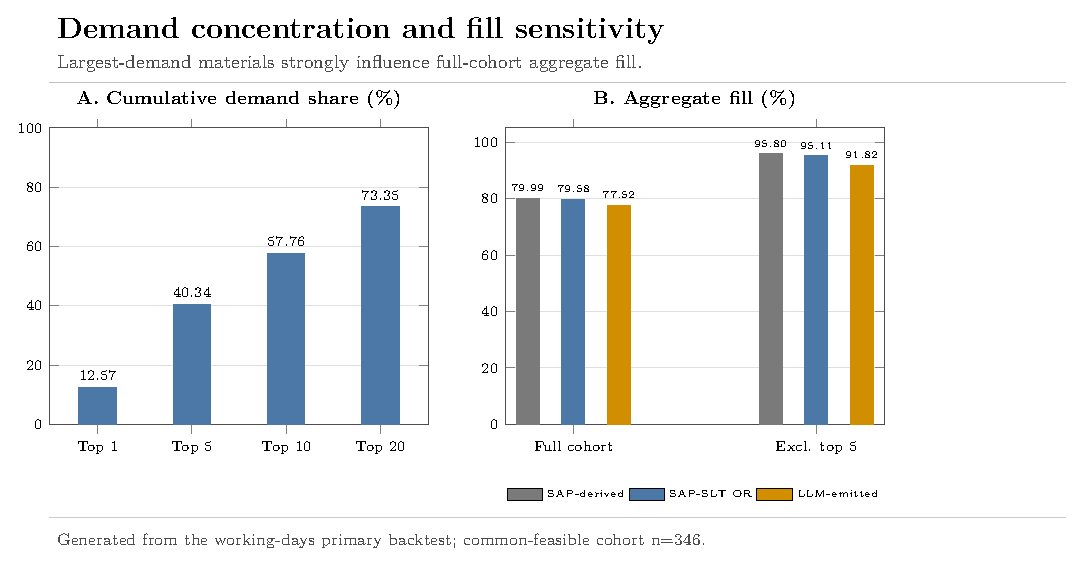
\includegraphics[width=0.98\linewidth]{Figure_2_Comparison.pdf}
\caption{Demand concentration and aggregate-fill sensitivity. Panel A reports cumulative demand share for the largest materials. Panel B compares full-cohort aggregate fill with the value after excluding the five largest-demand materials.}
\label{fig:publication-summary-graphics}
\end{figure}

Relative to SAP-derived, LLM-emitted policies have 2.48 percentage points lower aggregate fill, 335.24 lower mean holding/order cost, and 195 additional stockout days. Relative to SAP-SLT-informed OR, they have 2.07 percentage points lower aggregate fill, 1{,}003.26 lower mean holding/order cost, and 137 additional stockout days. These values describe one simulated cohort, not a definitive ranking or an economic preference.

Aggregate evidence is demand-concentrated. The largest 1, 5, 10, and 20 materials contribute 12.57\%, 40.34\%, 57.76\%, and 73.35\% of post-cutoff demand. Excluding the five largest-demand materials raises aggregate fill to 91.82\% for LLM-emitted, 95.80\% for SAP-derived, and 95.11\% for SAP-SLT-informed OR, versus 77.52--79.99\% in the full cohort (Figure~\ref{fig:publication-summary-graphics}). Thus, the largest-demand items drive aggregate fill and should not be obscured by cohort averages.

At material level, LLM-emitted fill is not lower than SAP-derived for 314 of 346 materials (90.8\%), while its cost is no higher for 238 (68.8\%); both conditions hold for 211 (61.0\%). Against SAP-SLT-informed OR, the corresponding counts are 309 (89.3\%), 303 (87.6\%), and 269 (77.7\%). Paired LLM-minus-comparator fill differences have first quartile, median, and third quartile of 0.00 percentage points for both comparators, reflecting many exact fill ties. Corresponding cost differences are $-259.24$, $-47.17$, and $34.96$ versus SAP-derived and $-787.83$, $-209.32$, and $-25.26$ versus SAP-SLT-informed OR. A deterministic 10{,}000-resample paired bootstrap gives LLM-minus-SAP fill and cost means of $-0.44$ percentage points (95\% interval $[-0.99,-0.02]$) and $-335.24$ (95\% interval $[-629.16,-105.29]$); against SAP-SLT-informed OR, the corresponding values are $-0.33$ percentage points ($[-0.89,0.14]$) and $-1{,}003.26$ ($[-1{,}363.81,-705.03]$). These descriptive resampling intervals and aggregate results jointly show service--cost trade-offs rather than uniform policy ranking.

The artifact audit covers all 365 scoreable policies: normalized policy-family agreement is 90.68\%, and 42 artifacts meet a prespecified diagnostic-outlier rule (CV absolute error above 0.75 or LLM-to-pipeline safety-stock ratio outside [0.5, 2.0]). Removing the 23 flagged artifacts present in the common cohort raises LLM aggregate fill from 77.52\% to 79.55\%, while SAP-derived reaches 80.08\% and SAP-SLT-informed OR reaches 79.70\%; this post-hoc diagnostic subset does not establish a causal correction. Replacing primary working-day receipt offsets with calendar-day offsets gives aggregate fills of 77.77\%, 80.25\%, and 79.84\%, respectively. Removing the one plant whose source working-day flags are entirely absent, and whose calendar is therefore imputed, leaves 280 native-calendar pairs with aggregate fills of 74.03\% for LLM-emitted, 76.55\% for SAP-derived, and 76.35\% for SAP-SLT-informed OR, mean material-level fills of 98.19\%, 98.71\%, and 98.54\%, zero-stockout shares of 81.79\%, 88.21\%, and 90.71\%, and mean holding/order costs of 2{,}893.68, 3{,}471.66, and 4{,}168.76. In this native-calendar subset both comparators retain higher fill and higher zero-stockout shares than the LLM arm, so the imputed calendar does not manufacture the observed service gap. With a lost-sales penalty of one times unit cost, mean total costs are 1{,}688{,}922.75, 1{,}631{,}321.28, and 1{,}692{,}746.91, respectively; at five times unit cost, they are 8{,}433{,}217.92, 8{,}143{,}869.56, and 8{,}448{,}325.64. Thus, zero-penalty holding/order cost cannot establish economic superiority. These sensitivities do not resolve empty-pipeline, excluded-flow, or calendar-repair limitations.

\section{Discussion}
\label{sec:discussion}

The current results document an applied AI/OR prototype on one anonymized industrial dataset. The LLM artifacts are generated from cutoff-bounded, pre-cutoff material histories, and all arms use the same post-cutoff horizon. The SAP-SLT-informed OR comparator is not independent of ERP inputs. The comparison remains descriptive rather than a controlled prospective trial: the 365-material artifacts support auditing and code-path verification, while the 346-pair common-feasible cohort supports no definitive performance ranking.

One structural asymmetry limits how the observed service gap may be interpreted. Both comparator arms are warm-started from ERP settings that already embed accumulated planner judgment: the SAP-derived arm retains the source SAP safety stock and recomputes only the reorder point and order quantity, and the SAP-SLT-informed OR arm consumes the source SAP safety-lead-time field. The LLM arm, by contrast, receives only a material-scoped history and a parameter block and must construct every policy value from that evidence alone. The observed aggregate-fill deficit of roughly two percentage points is therefore a warm-start versus cold-start comparison, not a like-for-like contest between a generator and an optimizer at equal information. An ERP-independent cold-start OR arm, computing safety stock from pre-cutoff demand and lead-time statistics without any source safety-stock or safety-lead-time input, is the comparator required to isolate generator quality; it is not available in the present release and is listed among the future-work requirements.

InventOR makes the input, artifact, and evaluation boundary inspectable without making LLM inference deterministic \cite{amershi2019guidelines, wasserkrug2025enhancing}. An aggregate-only manifest hashes the active input, evaluation code, and stored artifacts, while explicitly identifying unavailable deployed prompt, application, model/runtime, setting, and timestamp records. A stored input, artifact, and simulator version reproduce a recorded result; a fresh completion may vary. The tracked historical 315-material snapshots are byte-identical rather than distinct generation replicates, so they cannot estimate generation variance. Missing-output lists, parser checks, retries, and material-level simulation rows keep incomplete execution visible \cite{raji2020accountability, ouyang2025nondeterminism}. The workflow avoids project-specific training, but offers no evidence on setup effort, inference cost, or planner adoption.

The accepted policies satisfy a per-material storage bound, not a joint capacity constraint. They do not model shared capacity, substitution, or coordinated ordering. Their service--cost trade-off is not a replacement recommendation; a prospective trial with economically grounded shortage costs, repeated inference, and enforced planner review is required before adoption \cite{silver2017inventory, prak2021robust}.

Several limitations delimit the conclusions. All comparisons remain descriptive simulations; the paired bootstrap intervals characterize resampling variation across this cohort, not repeated LLM inference or a causal effect. Evidence comes from one anonymized dataset, one horizon, and one preserved full-cohort LLM generation; fresh completions may vary. An earlier unconstrained 315-material artifact set is retained for provenance, but its different cohort and validation end date preclude attributing differences to the storage rule. Demand is concentrated, with the five largest materials representing 40.34\% of demand. The calendar-day-arrival, lost-sales-penalty, and diagnostic-outlier sensitivities are limited checks, not replacements for a pipeline or flow-data reconstruction. The simulation begins with observed on-hand inventory but no outstanding-order pipeline and excludes observed receipts, corrections, and scrap. Plant C's working-day calendar is reconstructed from other plants; the native-calendar subset excludes it, but no independently validated Plant C calendar is available. The SAP-SLT-informed OR arm retains an SAP input, and the LLM receives SAP reference context; neither comparator establishes independent incumbent-SAP performance. The capacity rule is per material and does not model shared capacity, substitution, multi-echelon interactions, or coordinated ordering \cite{clark1960multi, federgruen1984allocation}. Recommendation quality remains dependent on data quality, historical representativeness, application configuration, and policy conversion rules \cite{kang2005information, watts2009data}. Narrative completeness and planner effectiveness were not evaluated.

These limitations define the scope for future work: a prospective evaluation that freezes the deployed configuration and model/runtime identifiers, repeats inference, initializes the replenishment pipeline, validates lead-time and calendar semantics, includes unchanged incumbent and ERP-independent comparators, estimates economically grounded shortage costs, reports first-pass reliability, and extends to multi-item and shared-capacity settings with planner review. The present evidence supports a prototype with traceable inputs, stored artifacts, and deterministic simulation; it does not support a controlled-trial comparative performance claim \cite{tashman2000out, hewamalage2023forecast}.

\section{Conclusion}
\label{sec:conclusion}

This paper presents \emph{InventOR}, an applied AI/OR prototype that treats LLMs as candidate-policy generators within deterministic preparation, parsing, and simulation. The framework preserves an inspectable link between material histories, policy fields, and simulated outcomes without project-specific model training or fine-tuning.

The executed artifact set contains 365 scoreable policies generated from cutoff-bounded, pre-cutoff material histories. Every accepted LLM policy satisfies its material-level storage bound. On the 346-pair cohort where all arms satisfy identical MOQ and supplied storage rules, LLM-emitted aggregate fill is 77.52\%, mean material-level fill is 97.94\%, mean simulated material-horizon holding/order cost is 2{,}848.96, and stockout days total 936 under working-day receipt scheduling. Positive shortage-cost sensitivities remove the apparent cost advantage. These values are descriptive simulated-comparison evidence, not repeated-inference or controlled prospective-trial evidence. The framework establishes a reviewable prototype and protocol for subsequent prospective evaluation, not a deployment or adoption claim.

\section*{Author Contributions}
Conceptualization, Methodology, Software, Formal analysis, Validation, Visualization, Writing -- original draft, Writing -- review and editing: Aris Dressino.

\section*{Funding}
This research did not receive any specific grant from funding agencies in the public, commercial, or not-for-profit sectors.

\section*{Declaration of Competing Interest}
The author declares no known competing financial interests or personal relationships that could have appeared to influence the work reported in this paper.

\section*{Data and Code Availability}
The raw operational data and material-level artifacts cannot be publicly released because they contain commercially sensitive material, supplier, and planning information. A confidentiality-screened release package containing analysis code, the anonymized variable schema, aggregate evaluation results, manuscript sources, and aggregate integrity manifest is available at \texttt{github.com/DressPD/inventor\_public}. The release package is additionally deposited in a Zenodo archive whose version-specific DOI will be registered at acceptance and cited in the final version of record; the GitHub repository is the development mirror and the Zenodo deposit is the citable archival copy. Supplementary File S1 accompanies this submission and contains the intended application-side prompt specification. The historical deployed application configuration, model/runtime identifier, inference dates, and prompt hashes were not preserved and are not claimed as available; the current runner records these fields for future executions.

\section{Acknowledgments}
\label{sec:ack}

The author thanks the industrial collaborators and material-control experts who contributed domain knowledge and access to anonymized operational data. The author also acknowledges the associated enterprise data and IT teams for supporting data access and prototype execution. No formal full-population planner evaluation is claimed. Any errors or omissions remain the responsibility of the author.

\section*{Declaration of Generative AI and AI-Assisted Technologies in the Writing Process}
During manuscript preparation, the author used OpenAI GPT-5.6 through OpenCode for language editing, consistency checks, citation review, and LaTeX proofing support; this is a writing-assistance tool and is distinct from the Anthropic Claude Sonnet 4.6 deployment evaluated in the research workflow. The author reviewed and edited the content after use and takes full responsibility for the content of the published article. Figures were rendered deterministically from author-reviewed LaTeX and Python source; generative AI did not directly create or manipulate image content. The research workflow evaluated in the paper is itself the object of study and is described separately in the methodology.

%% If you have bib database file and want bibtex to generate the
%% bibitems, please use
%%
\begingroup
\small
\bibliographystyle{elsarticle-num}
\bibliography{refs}
\endgroup

\end{document}

\endinput
%%
%% End of InventOR manuscript.
